\section{Case Study}
\label{ap:case_study}

\addtocontents{toc}{\protect\setcounter{tocdepth}{1}}


\begin{figure*}[t]
\centering
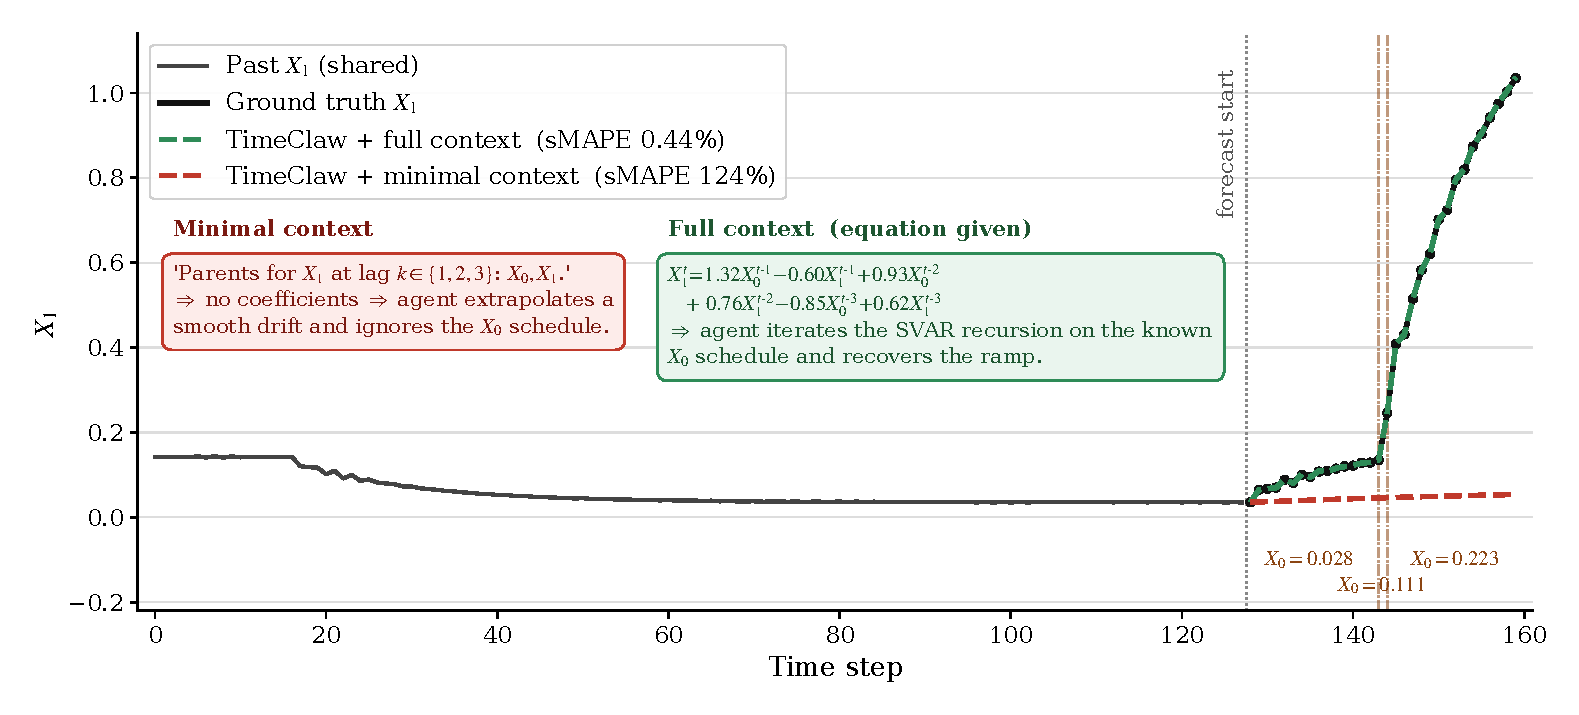
\includegraphics[width=\linewidth]{figures/cik_case_study_svar.pdf}
\caption{Case study on a paired SVAR task from Context-is-Key \citep{DBLP:conf/icml/WilliamsAMZSRRL25}. Given identical history and ground truth, \method{} recovers the ramp when the prompt contains the SVAR equation and misses it entirely when only the qualitative parent list is provided. This demonstrates that \method{} actively grounds its forecast in the textual context, rather than extrapolating from the numerical history alone.}
\label{fig:cik_case}
\vspace{-3mm}
\end{figure*}




\subsection{How \method Leverages Context?}

To test how \method{} leverages textual context rather than
pattern-matching on numerical history, we pair two SVAR tasks at the same
seed: \textsc{MinimalCausalContextBivarLinSVAR} and
\textsc{FullCausalContextExplicitEquationBivarLinSVAR}. The two records
have byte-identical 128-step past history of $X_1$, identical 32-step
ground truth, and the same step-change schedule for the covariate $X_0$
($0.028\!\to\!0.111\!\to\!0.223$). The Minimal prompt only lists the
qualitative parents of $X_1$; the Full prompt additionally spells out the
linear SVAR equation with all six coefficients. Any difference in
forecast quality must therefore route through the agent's reading of
roughly $400$ extra tokens of context.

Figure~\ref{fig:cik_case_study_svar} overlays both forecasts on the
shared ground truth. Given the equation, the agent inspects recent $X_1$
values through the analysis tools and unrolls the SVAR recursion on the
known future $X_0$ schedule, recovering the ramp from $0.035$ to $1.03$
within $\sim\!10^{-3}$ (sMAPE $\mathbf{0.44\%}$). Without the
coefficients it cannot translate the $X_0$ jumps into $X_1$ movements
and falls back to a smooth drift inside $[0.036, 0.054]$, missing the
ramp entirely (sMAPE $\mathbf{124\%}$). The $\sim$280 times gap on
identical numerical inputs confirms that, when context carries
decision-relevant structure, \method{} propagates that structure into
the forecast rather than relying on the history alone.




\begin{figure*}[h]
\centering
\begin{subfigure}[t]{0.32\textwidth}
  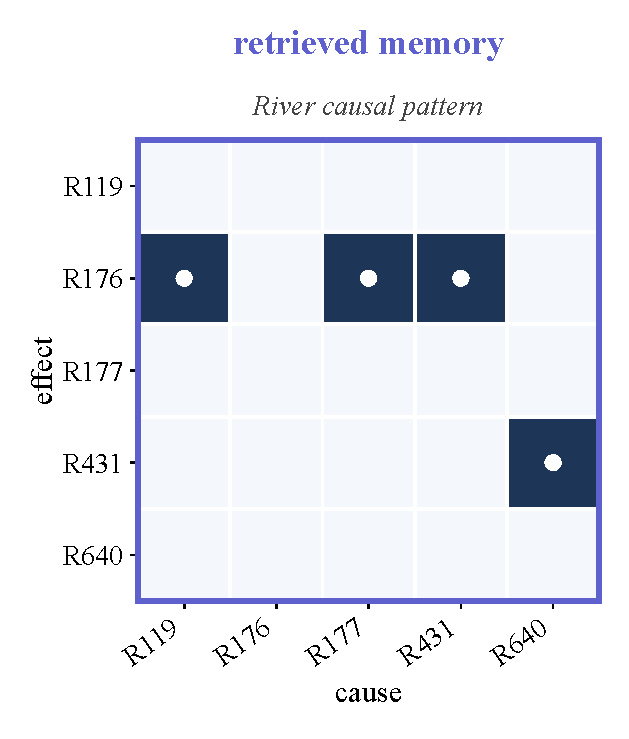
\includegraphics[width=\linewidth]{figures/tsrbench_case_study_causal_retrieved.pdf}
\end{subfigure}\hfill
\begin{subfigure}[t]{0.32\textwidth}
  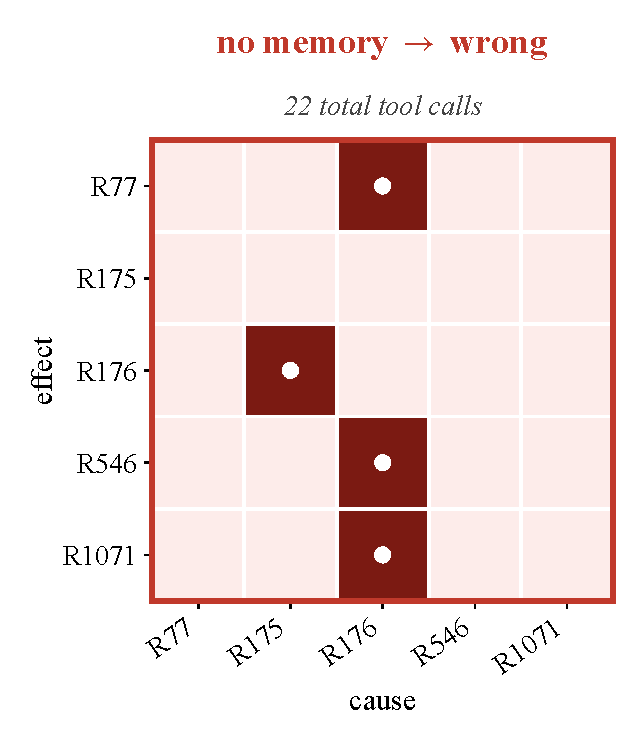
\includegraphics[width=\linewidth]{figures/tsrbench_case_study_causal_k0_wrong.pdf}
\end{subfigure}\hfill
\begin{subfigure}[t]{0.32\textwidth}
  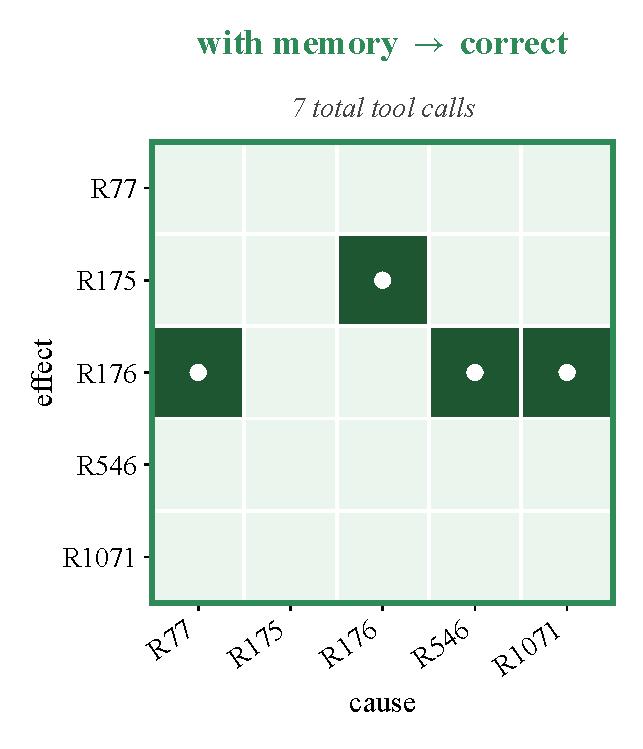
\includegraphics[width=\linewidth]{figures/tsrbench_case_study_causal_k3_correct.pdf}
\end{subfigure}
\caption{
Causal maps of the case study on memory transfer in TSRBench river flood causal reasoning (R stands for "River"). 
\textbf{Left:} a retrieved memory summarizes an upstream-to-downstream cascade from a related but different river system, providing a transferable structural rule. 
\textbf{Middle:} without memory, the agent performs broad exploratory analysis and commits to a physically reversed adjacency after $22$ tool calls. 
\textbf{Right:} with memory, the agent reuses the retrieved upstream-to-downstream reasoning pattern, executes only $7$ targeted tool calls, and selects the correct causal structure. 
This illustrates that episodic memory improves reasoning by transferring compact task-level rules across related temporal scenarios, rather than by matching numerical histories alone.
}
\label{fig:tsrbench_case_study_causal}
\end{figure*}




\subsection{How Task Memory Steers Agent Decisions}

To examine how retrieved task memory changes agent behavior, we trace
\method{} on a representative TSRBench causal-reasoning instance. The task asks
the agent to infer the causal adjacency among multiple river sensors from the
same underlying time series. We run the task under two settings with the same
agent, MCP tool budget, and numerical input: retrieval disabled ($k\!=\!0$) and
top-$3$ memory retrieval enabled ($k\!=\!3$). The retrieved memories come from
the training bank and do not overlap with the test split.

Figure~\ref{fig:tsrbench_case_study_causal} contrasts the two outcomes. 
Without memory, the agent performs a broad numerical sweep, issuing $22$ tool
calls across \texttt{channel\_stats}, \texttt{compute\_acf},
\texttt{find\_peaks}, and \texttt{detect\_periodicity} for all channels.
Despite this exhaustive inspection, it selects a physically reversed causal
structure, mistaking downstream effects for upstream causes. 

With memory, retrieval returns related causal-reasoning trajectories from
sibling tasks. One retrieved memory summarizes a transferable rule: the relevant
mechanism follows an upstream-to-downstream cascade. Guided by this rule, the
agent avoids an exhaustive scan, runs only $7$ targeted \texttt{compute\_acf}
probes to verify the lead-lag pattern, and selects the correct adjacency. 
Importantly, the retrieved memory provides no additional observations from the
test instance; it transfers a compact decision rule learned from a different
river system. Thus, memory changes both the answer and the reasoning process,
reducing the tool budget by over $3\times$ while steering the agent toward the
correct causal direction. A step-by-step trace is provided in
Figure~\ref{fig:tsrbench_case_study_causal_box}.








\subsection{How \method{} Evolves New Tools from Experience?}

We further examine how \method{} expands its toolset through experience-driven capability evolution. 
Tool evolution converts recurring successful trajectories into reusable executable routines. 
This mechanism is especially useful when the initial toolbox only provides generic time-series operations, while a benchmark repeatedly requires domain-specific computations that are cumbersome or unreliable to reconstruct from low-level tools. 
In such cases, \method{} summarizes successful training trajectories, identifies repeated analytical routines, and promotes them into callable tools with standardized argument schemas. 
The evolved tools can then be reused at test time, allowing the agent to bypass brittle manual arithmetic and directly execute the intended computation.

Figure~\ref{fig:tsaia_case_study_finance_tools} illustrates this process on TSAIA's finance split. 
Starting from a generic time-series toolbox, the agent observes recurring successful trajectories involving portfolio risk-adjusted return estimation, portfolio risk estimation, and market-factor regression. 
From these trajectories, \method{} evolves three finance-specific tools: \texttt{portfolio\_sharpe}, \texttt{portfolio\_var}, and \texttt{capm\_regression}. 
At test time, these evolved tools provide direct executable support for financial reasoning, improving both accuracy and tool-use efficiency. 
This case study shows that capability evolution transfers reusable computational procedures, rather than task-specific data, and enables the agent to acquire new domain-specific skills from prior experience.













\section{Prompt Templates}
\label{app:prompts}

\method instantiates a small family of prompts that share the same high-level
skeleton but specialize the input rendering, the output schema, and the
tool-use guidance to the underlying benchmark. All test-time prompts can
optionally be wrapped with a retrieval prefix that injects top-$k$ trajectory
summaries from the episodic memory bank, and all training-time prompts are
extended with a ground-truth-aware suffix that elicits a transferable
\texttt{<context\_to\_action>} explanation block. We describe the unified
skeleton in Figure~\ref{fig:prompt_template_general}, and an example per-benchmark
instantiations in Figure~\ref{fig:prompt_tsrbench}. We further describe the memory bank prompt in Figure ~\ref{fig:prompt_augments}.



\clearpage


\begin{figure*}[h]
\centering
\resizebox{\textwidth}{!}{
\begin{tcolorbox}[colback=gray!5!white, colframe=pink!120,
title=Case Study C.1: \method{} on Context-is-Key: How Textual Context Steers the Forecast,
boxrule=0.3mm, width=1.2\textwidth, arc=2mm, auto outer arc=true]

\textbf{Core Task.}
We pick a pair of CiK tasks from the bivariate linear SVAR family at the
same seed (\texttt{seed=5}): \textsc{MinimalCausalContextBivarLinSVAR} and
\textsc{FullCausalContextExplicitEquationBivarLinSVAR}. The two records
share \emph{identical} 128-step past history and 32-step ground-truth
future of the target variable $X_1$, and share the same step-change
schedule for the covariate $X_0$ over the forecast window
($0.028 \!\to\! 0.111 \!\to\! 0.223$). The \emph{only} difference is what
the textual context reveals about the data-generating process. This
isolates a clean variable: context $\to$ forecast.

\vspace{2mm}

\textbf{Prompt:} See Appendix~\ref{app:prompts} for the full prompt template.

\vspace{2mm}

\textbf{Visualization:} We provide Figure \ref{fig:cik_case} to better illustrate this case study.

\vspace{3mm}
\hrule
\vspace{3mm}

\textbf{Memory Retrieval Stage.}
\begin{enumerate}
    \item \textbf{Two-stage retrieval.}
    \method{} embeds the task's
    \texttt{background + scenario + constraints} block with
    \texttt{text-embedding-3-small}, takes the top-$K_{\text{text}}$ records
    by cosine similarity from the training bank, then re-ranks the
    survivors by L2 distance on the 20-dim numerical fingerprint of
    \texttt{past\_time}. With $k\!=\!1$ on this task both stages converge
    on the same family (\textsc{FullCausalContextImplicitEquationBivarLinSVAR})
    seen during training.

    \item \textbf{Reference compression.}
    The retrieved trajectory is compressed by \texttt{summarize\_trajectory} into the trainer's analytic spine: a \texttt{context$\to$forecast} explanation, together with the sequence of MCP tool calls and their truncated responses. 
    This summary is then injected before the test prompt as a \texttt{REFERENCES FROM PRIOR TRAINING} block, surfacing the transferable rule that the scenario's lagged linear parent effects should be handled by iterating the SVAR recursion over the known future $X_0$ schedule.
\end{enumerate}

\textbf{Execution Stage (Full Context).}
\begin{enumerate}
    \item \textbf{Context parsing.}
    The agent reads the explicit linear SVAR equation from the prompt
    ($X_1^{t} = 1.322\,X_0^{t\text{-}1} - 0.604\,X_1^{t\text{-}1} +
    0.926\,X_0^{t\text{-}2} + 0.763\,X_1^{t\text{-}2} -
    0.851\,X_0^{t\text{-}3} + 0.623\,X_1^{t\text{-}3}$) and the
    piece-wise constant schedule for $X_0$ over the 32-step horizon.

    \item \textbf{Tool-grounded historical inspection.}
    Guided by the retrieved spine, the agent invokes the MCP analysis
    server: \texttt{series\_overview()} $\to$ \texttt{channel\_stats("1")}
    $\to$ \texttt{compute\_acf("1", max\_lag=20)} $\to$ \texttt{channel\_values("1", 120, 128)},
    confirming the recent $X_1$ levels needed to seed the recursion.

    \item \textbf{Closed-form forecast.}
    With the equation, the recent lagged values, and the future $X_0$
    schedule all known, the agent unrolls the recursion deterministically,
    producing a 32-step forecast that tracks the ground-truth ramp from
    $0.035 \!\to\! 1.03$ almost exactly.
\end{enumerate}

\textbf{Counterfactual: Minimal Context, Same Series.}
On the matched \textsc{Minimal}-context variant, the prompt only states that
``parents for $X_1$ at lag $k\!\in\!\{1,2,3\}$ are $X_0, X_1$,'' while the
six SVAR coefficients are withheld. 
Given the same retrieved memory and tool budget, the agent cannot reconstruct the
recursion and instead falls back to extrapolating a small monotone drift in
$[0.036, 0.054]$, missing the $X_0$ step changes that drive the true ramp.

\vspace{2mm}
\textbf{Evaluation.}
On the full-context variant, \method{} achieves \textbf{sMAPE 0.44\%}
(MSE $\approx\!10^{-6}$), compared with \textbf{sMAPE 124\%}
(MSE $0.254$) on the minimal-context variant. 
This yields a $\sim\!280\times$ sMAPE gap for forecasting the
\emph{same} numerical series. 
Since the two variants share identical histories, retrieved memory, and tool
budget, the gap is explained by the $\sim\!400$-token difference in textual
context. 
This demonstrates that \method{}'s gains arise from context comprehension rather
than distributional pattern matching on the history alone. 
Figure~\ref{fig:cik_case_study_svar} overlays both forecasts on the shared past
and ground truth.

\end{tcolorbox}}
\caption{
Case study of \method{} on a pair of CiK SVAR tasks that share their
numerical history and ground truth but differ only in the textual
description of the data-generating process. With the explicit SVAR
equation in context, the agent iterates the recursion on the known $X_0$
step schedule and recovers the ground-truth ramp (sMAPE $0.44\%$). With
only a qualitative parent list, it extrapolates a smooth low-amplitude
drift and misses the ramp entirely (sMAPE $124\%$). The two annotated
boxes inside the panel reproduce the exact context delta between the two
prompts.
}
\label{fig:cik_case_study_svar}
\end{figure*}






\clearpage




\begin{figure*}[h]
\centering
\resizebox{\textwidth}{!}{
\begin{tcolorbox}[colback=gray!5!white, colframe=brown!55,
title=Case Study C.2: \method{} on TSRBench: How Retrieved Memory Steer the Decision,
boxrule=0.3mm, width=1.2\textwidth, arc=2mm, auto outer arc=true]

\textbf{Core Task.}
A multiple-choice causal-discovery question from TSRBench (\texttt{causal\_reasoning}, Elbe-River-Flood). The agent is shown $64$ days of runoff measurements from five river sensors and must pick the $5\!\times\!5$ binary adjacency matrix that captures the causal structure (columns = cause, rows = effect). Ground-truth answer is D: an upstream-to-downstream cascade in which small tributaries (rivers R77, R546, R1071) feed the large downstream river R176, which in turn feeds R175.

\vspace{2mm}

\textbf{Prompt:} See Appendix~\ref{app:prompts} for the full template.

\vspace{2mm}
\textbf{Visualization:} We provide Figure \ref{fig:tsrbench_case_study_causal} to better illustrate this case study.

\vspace{3mm}
\hrule
\vspace{3mm}

\textbf{Memory Retrieval Stage.}
\begin{enumerate}
    \item \textbf{Two-stage retrieval.}
    \method{} embeds the test prompt with \texttt{text-embedding-3-small} and selects the top-$K_{\text{text}}$ records from the training bank by cosine, then re-ranks the survivors by $L2$ distance on the fingerprint of the loaded series. Then \method retrieves $k\!=\!3$ records.
    % sibling Elbe-flood tasks defined over different river subsets.

    \item \textbf{Rule extraction via \texttt{summarize\_trajectory}.} Each retrieved trajectory is compressed to a tool-call spine plus a \texttt{context\_to\_action} block written during training. One block of the retrieved action in memory reads verbatim: \emph{``the mechanism mapping is upstream-to-downstream edges.''} This is the transferable decision rule that primes the test agent.

    \item \textbf{Prompt injection.}
    The compressed references are concatenated as a \texttt{REFERENCES FROM PRIOR TRAINING} block in front of the test prompt, only analytic spine and decision rules.
\end{enumerate}

\textbf{Execution Stage.}
\begin{enumerate}
    \item \textbf{Targeted tool use.}
    Primed by the retrieved rule, the agent runs only the inspections needed to confirm direction: \texttt{list\_channels} $\to$ \texttt{series\_overview} $\to$ five \texttt{compute\_acf} probes, one per river. It skips the exhaustive per-channel statistics, peak-finding, and periodicity-detection that the no-memory agent runs through.

    \item \textbf{Mapping the rule onto the new river set.} The agent matches its own observations to the retrieved rule: the channels with mean flow $\sim\!660$--$680$ (R175, R176) form the downstream sinks; the three with mean flow $<\!4$ (R77, R546, R1071) are upstream tributaries. The rule then determines option D, in which the sink row R176 is densely populated with parents from the tributaries and the tributaries themselves are source rows.

    \item \textbf{Answer realisation.} The agent emits the final letter \texttt{<answer>D</answer>}, with a brief justification citing the retrieved cascade rule.
\end{enumerate}


\textbf{Counterfactual: Same Series, No Memory.}
Re-running the identical task at $k\!=\!0$ removes only the \texttt{REFERENCES} block. Without memory, the agent resorts to brute-force inspection, issuing $22$ tool calls across \texttt{channel\_stats}, \texttt{compute\_acf}, \texttt{find\_peaks}, and \texttt{detect\_periodicity} for every channel. It then selects option A, which encodes the physically reversed cascade (R176 caused by R175; R77, R546, and R1071 each caused by R176). Without the retrieved rule, the agent lacks an anchor for causal direction and defaults to a topology inconsistent with the observed lead-lag patterns.

\vspace{2mm}
\textbf{Evaluation.} On the same instance, \method{} changes from \textbf{wrong (A)} at $k\!=\!0$ (without memory) to \textbf{correct (D)} at $k\!=\!3$ (with memory), while reducing the tool-call budget from $22$ to $7$ ($3.1\!\times$ fewer calls). 
The retrieved memory provides a transferable \emph{decision rule}. 
This demonstrates memory improves reasoning by carrying compact rules that redirect the agent's search process, rather than by matching numerical histories alone.


\end{tcolorbox}}
\caption{Case study on a TSRBench river-flood causal-discovery instance}
\label{fig:tsrbench_case_study_causal_box}
\end{figure*}










\begin{figure*}[h]
\centering
\resizebox{\textwidth}{!}{
\begin{tcolorbox}[colback=gray!5!white, colframe=violet!45,
title=Case Study C.3: \method{} on TSAIA: Finance Tools Evolved from Experienced Trajectories,
boxrule=0.3mm, width=1.2\textwidth, arc=2mm, auto outer arc=true]

\textbf{Core Task.}
TSAIA's finance split presents the agent with portfolio and market time-series panels and asks it to answer quantitative multiple-choice questions. At the beginning, the agent's toolbox only contains generic time-series inspection tools. It does not include finance-specific primitives for portfolio evaluation or market-factor regression. 
% As a result, a zero-shot agent must rely on generic statistics and manual arithmetic, which is brittle for tasks requiring precise financial computation.

\vspace{2mm}

\textbf{Prompt:} See Appendix~\ref{app:prompts} for the full template.

\vspace{3mm}
\hrule
\vspace{3mm}

\textbf{Tool Evolution.}
\begin{enumerate}
    \item \textbf{Routine extraction via \texttt{summarize\_trajectory}.}
    During training, three recurring analytical routines appear across successful trajectories: portfolio risk-adjusted return estimation, portfolio risk estimation, and market-factor regression. 
    Each successful trajectory is summarized into a compact routine description that records the input conventions, intermediate computations, and final decision rule. 
    These summaries reveal reusable computation patterns.

    \item \textbf{Evolving finance-specific tools.}
    From these recurring routines, \method{} evolves three finance-specific
    tool schemas and adds them to the agent's reusable toolbox:
    \vspace{-1mm}
    \begin{itemize}\setlength\itemsep{0pt}
      \item \texttt{portfolio\_sharpe(channels, weights, risk\_free, period\_per\_year)}: compute risk-adjusted return for each
        portfolio option and compare the returned ratios.
      \item \texttt{portfolio\_var(channels, weights, horizon=$H$, alpha=$\alpha$, method="parametric")}: compute portfolio risk using task metadata and compare the resulting losses across options.
      \item \texttt{capm\_regression(asset\_channel, market\_channel)}: estimate market-factor statistics $\{\alpha,\beta,r^{2}\}$ and select the option whose target statistic matches the returned value.
    \end{itemize}
\end{enumerate}
\textbf{Evaluation.}
Across the finance test split, evolved tools improve both accuracy and tool-use efficiency, especially when manual arithmetic is unreliable. On {MarketAB-beta} tasks, the average number of \texttt{capm\_regression} calls per task increases to $0.83$, and accuracy rises by $+16.7$. On {VaR} tasks, accuracy improves by $+12.0$, while the average tool budget drops from $6.3$ to $5.2$.

\end{tcolorbox}}
\caption{
Case study of \method{} on TSAIA's finance MC split. 
Starting from a generic time-series toolbox, \method{} observes recurring
successful training trajectories and evolves finance-specific tools for
portfolio evaluation and market-factor regression. 
At test time, these evolved tools replace brittle manual arithmetic with
direct executable routines, improving accuracy while reducing unnecessary
exploratory calls. 
}
\label{fig:tsaia_case_study_finance_tools}
\end{figure*}












\clearpage

% =====================================================================
% B.1  General template
% =====================================================================
\begin{figure*}[h]
\centering
\resizebox{\textwidth}{!}{
\begin{tcolorbox}[
colback=gray!5!white, colframe=blue!70,
title=Prompt Template B.1: General Skeleton,
boxrule=0.3mm, width=1.2\textwidth, arc=2mm, auto outer arc=true]

\textbf{General Prompt.} All \method prompts decompose the input into a fixed
sequence of optional slots: a retrieval prefix, a tool-use hint (when the
agent is wired to the MCP analysis server), a benchmark-specific header, the
task question, an inline data block (only when the data is not preloaded
into the MCP server), an option list (for multiple-choice tasks), an
output-format clause, and a training-mode suffix. Concrete builders fill or
omit each slot according to the task type.

\begin{quote}
\texttt{\{retrieval\_prefix\}}

\texttt{\{tools\_hint\}}

\texttt{\{header\}}

\medskip
\texttt{\{question\_or\_context\}}

\medskip
\texttt{\{inline\_data\_block\}}

\medskip
\texttt{\{options\}}

\medskip
\texttt{\{output\_format\}}

\medskip
\texttt{\{training\_suffix\}}
\end{quote}

\textbf{Template fields.}
\texttt{\{retrieval\_prefix\}} is the optional ``REFERENCES FROM PRIOR
TRAINING'' block (Fig.~\ref{fig:prompt_augments}, left), inserted at test
time when the memory bank returns nearest-neighbor trajectories.
\texttt{\{tools\_hint\}} reminds the agent which MCP analysis tools are
available and the recommended inspection pattern.
\texttt{\{header\}} carries benchmark-level metadata.
\texttt{\{question\_or\_context\}} contains the task statement (TSRBench /
TSAIA) or the textual context fields (CiK).
\texttt{\{inline\_data\_block\}} renders the partial numerical series as text when needed, and is
often suppressed, since the canonical data is preloaded
into the MCP server.
\texttt{\{options\}} is the lettered option list only for multiple-choice tasks.
\texttt{\{output\_format\}} pins the response schema.
\texttt{\{training\_suffix\}} is the optional extension
(Fig.~\ref{fig:prompt_augments}, right) that converts the prompt into a
trajectory-collection prompt during memory-bank construction.
\end{tcolorbox}}
\caption{
General prompt skeleton used in \method. A small set of optional slots
covers all benchmarks; each concrete builder fills the slots appropriate
to its task type and tool-availability regime.
}
\label{fig:prompt_template_general}
\end{figure*}


% =====================================================================
% B.2  TSRBench
% =====================================================================
\begin{figure*}[h]
\centering
\resizebox{\textwidth}{!}{
\begin{tcolorbox}[
colback=gray!5!white, colframe=blue!70,
title=Prompt Template B.2: TSRBench,
boxrule=0.3mm, width=1.2\textwidth, arc=2mm, auto outer arc=true]

\textbf{TSRBench Prompt.} TSRBench questions come in three surface forms:
(i)~``perception'' questions with an inline \texttt{<ts><ts/>} placeholder
where the series should be substituted, (ii)~multiple-choice questions with
a \texttt{choices} field, and (iii)~free-form questions. The same template
handles all three by toggling the rendering of the series block and the
options block; the answer schema is always a single
\texttt{<answer>...</answer>} tag.

\begin{quote}
\texttt{Domain: \{domain\}} \\
\texttt{Task type: \{task\}} \\
\texttt{Series names: \{names\}}

\medskip
% \textit{(tool-aware variant only)}\\
The numerical time series for this question is already loaded into your
analysis tool server. Inspect it with the available tools before answering.
A typical pattern: (1) \texttt{list\_channels()} / \texttt{series\_overview()};
(2) \texttt{channel\_stats} / \texttt{channel\_values} / \texttt{compute\_acf} /
\texttt{detect\_periodicity} / \texttt{find\_peaks} on individual channels.
Do NOT guess values you haven't retrieved through tools.

\medskip
\texttt{Question:} \\
\texttt{\{question\}}


\medskip
\textit{(MC subtasks only)}\\
\texttt{Options:} \\
\texttt{A. \{option\_A\}} \\
\texttt{B. \{option\_B\}} \\
\texttt{...}

\medskip
Reason carefully, then output your final answer wrapped exactly like this on
its own line: \texttt{<answer>X</answer>}. 
\end{quote}
\end{tcolorbox}}
\caption{
Specific TSRBench prompt template. For Context-is-Key and TSAIA prompt template, please refer to our code implementation. 
}
\label{fig:prompt_tsrbench}
\end{figure*}



% =====================================================================
% B.5  Augmentations: retrieval prefix + training suffix
% =====================================================================
\begin{figure*}[h]
\centering
\resizebox{\textwidth}{!}{
\begin{tcolorbox}[
colback=gray!5!white, colframe=blue!70,
title=Prompt Template B.3: Memory-Retrieval Prefix and Training-Mode Suffix,
boxrule=0.3mm, width=1.2\textwidth, arc=2mm, auto outer arc=true]

\textbf{Augmentation blocks.} Two cross-cutting blocks compose with every
builder above. The \textit{retrieval prefix} is inserted at test time when
the memory bank returns nearest-neighbor trajectories; the \textit{training
suffix} is appended at memory-bank-construction time so the agent produces
a justifying analytic trace plus a transferable
\texttt{<context\_to\_action>} explanation.

\begin{quote}
\textbf{Retrieval prefix (test time, when $k>0$ neighbors are retrieved):}

\texttt{=== REFERENCES FROM PRIOR TRAINING ===} \\
Below are similar prior tasks (same task family where possible) and how they
were solved, including which tools were called, the key numbers returned, and the
final answer. Use them as a guide for the analytic process. The correct
answer for the current task may differ; do not copy blindly.

\medskip
\texttt{Reference 1:} \\
\texttt{[family=<family\_key>]} \\
\texttt{\ \ <trainer's transferable explanation>} \\
\texttt{\ \ tool\_name(args) $\to$ <truncated\_response>} \\
\texttt{\ \ tool\_name(args) $\to$ <truncated\_response>} \\
\texttt{\ \ ...}

\medskip
\texttt{Reference 2: ...}

\medskip
\texttt{=== END REFERENCES ===}

\medskip\hrule\medskip

\textbf{Training-mode suffix (memory-bank construction):}

\texttt{TRAINING MODE}

\medskip
Do TWO things before emitting your final answer:

1. Inspect the series with whatever tools are available and walk through the
reasoning step by step.

2. Output a \texttt{<context\_to\_action>...</context\_to\_action>} block
($\leq$3 sentences) that explicitly states:
\begin{itemize}
\item which sentences in the context (background / scenario / constraints /
question / options) drive the answer's shape, AND
\item the rule that maps those sentences to that shape (e.g.\ ``scenario says
`heat wave for 2 hours' $\to$ ground truth has a 4$\times$ spike at the
stated start $\to$ because air-conditioning load scales with cooling
demand'').
\end{itemize}

Make this block transferable, NOT series-specific. Future test-time
agents will read it to map their own context, so avoid statements like ``the mean is 850'' and prefer statements like ``scenario X implies pattern Y because of mechanism Z''.

\medskip
Then produce your final answer in the format requested above.



\end{quote}
\end{tcolorbox}}
\caption{
The retrieval prefix (top) surfaces the
analytic spine of nearest-neighbor trajectories from the memory bank.
The training-mode suffix (bottom) is applied during the memory bank
construction, so the trainer agent produces the transferable explanation
block that the retrieval prefix later surfaces.
}
\label{fig:prompt_augments}
\end{figure*}

